\pagebreak
\section{Tombstone Diagram}
When developing a compiler, tombstone diagrams can be used to define the programming languages needed to compile the source code of a program. The tombstone diagram shows the source language, the language of the compiler(s), the language(s) of the different stages of compiling, and the target language.

\begin{figure}[H]
	\centering
		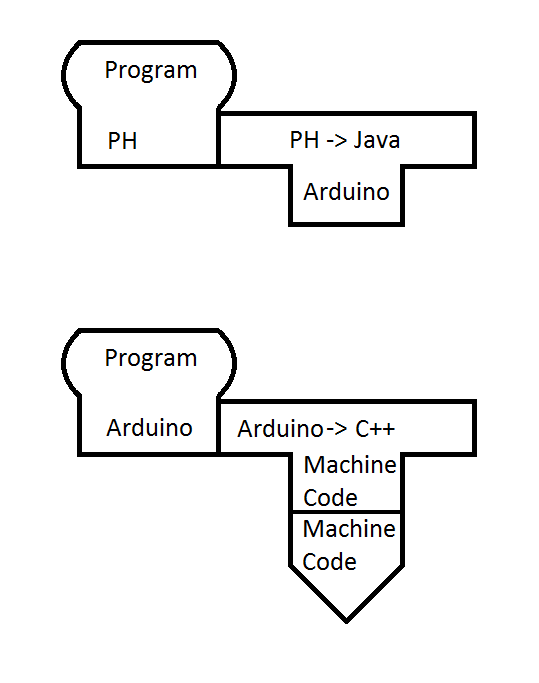
\includegraphics{billeder/tombstone_diagram.png}
		\caption{Tombstone diagram for the source language to machine code}
		\label{fig:tombstone}
\end{figure}

As seen in figure \ref{fig:tombstone} the tombstone diagram for this project is as follows: The program is written in BAL. It is then translated by the compiler (written in Java) into Arduino language. Since Arduino itself only understands machine code, another compiler (written in C++) is needed to translate from Arduino language into machine code. For this, the standard Arduino IDE is used.
Since this project focuses on compiling from BAL to Arduino language, the first tombstone diagram in figure \ref{fig:tombstone} is the important one in this project. Compiling from Arduino to machine code is done through Arduino's own software.